\chapter{Semi-parametric models}\label{semiparaGarch}

Parametric GARCH model has many advantages. The function form is accessible, and parameters could be easily estimated. If the model assumptions were correct, the estimation is consistent with reality. However, the drawbacks of parametric models are more disgusting. Firstly, a preselected parametric model may not fit unexpected features, due to too restricted or too low dimensional. Secondly, sometimes the regression function seems to be too complicate or difficult to be defined. Thirdly, because different sequence will be witnessed when different conditional distribution is selected in the process of prediction by using parametric models, there will most possibly exist the problem of misspecification,which may result in a excessively high model bias and loss of efficiency, unless the assumed function perfectly matches the true error distribution \citep{Di2011}.

Gourieroux and Monfort had firstly inserted the conditional mean and conditional vari-ance into a nonparametric model, in which the function form is not given. This model can supply the gaps of parametric models. Correspondingly, it is less sensitive to model misspecification and can offer a flexible tool in analyzing unknown regression relationships 
\citep{Gourieroux1992}. In nonparametric regression models, both the error distribution and the functional form of the mean function are not pre-specified. It will be more useful when the regression function seems to be very complex or a suitable function form cannot be found \citep{Eubank1993}. However, the nonparametric models lose some functions, which can be completed by parametric models. Due to lack of specific function forms, the parameters of the model cannot be estimated; further-more the model cannot be explained. Excess variable estimates could rise up because of poor consideration of nonparametric models, especially for small sample size. So a new model, semi-parametric model, is proposed.

Semi-parametric model consists of not only the nonparametric part but also parametric part. Semi-parametric GARCH model selects the nonparametric form for the scale func-tion and the parametric part for conditional variance lags. Then it does not need a pre-specified function form and is less sensitive to model misspecification. At the same time, the parametric part can also explain the models \citep{Di2011}.

\section{Semi-parametric GARCH model}

\subsection{Definition of semi- parametric GARCH model}

Semi-parametric GARCH model combines a smooth scale function with the standard GARCH model:

\begin{equation}
\label{eq:3.1}
Y_{t} = \mu + \sigma(x_{t})\varepsilon_{t}
\end{equation}

where $\mu$ is an unknown constant; $x_{t}=t/n; \sigma(x)>0$ is the nonparametric component, a smooth, bounded scale function; and $\lbrace\varepsilon_{t}\rbrace$ is the parametric component, which is assumed to follow a GARCH(p, q) process.

\begin{equation}
\label{equ3.3}
h_{t}=\omega + \sum_{i=1}^{p}\alpha_{i}\varepsilon_{t-i}^{2} + \sum_{j=1}^{q}\beta_{j}h_{t-j},
\end{equation}

where $h_t^{1/2}$ is the conditional standard deviations of the standardized process $\varepsilon_t$; $ \omega>0;  \alpha_{1}, \ldots ,\alpha_{p}\geq0$ and $\beta_{1},\ldots,\beta_{q}\geq0$.    To estimate the scale function, $E(\varepsilon_{t}^{8})<\infty$ is assumed to ensure \ref{equ3.3} strictly stationary, which implies in particular that $\sum_{i=1}^p\alpha_i+\sum_{j=1}^q\beta_j<1$ \citep{Feng2004}.

\subsection{Estimation of semi-parametric GARCH model}

The estimation of semi-parametric GARCH model can combine the nonparametric estimation of the Y's local variance  $v(x)=\sigma^{2}(x)$,with parametric estimation of the unknown parameter vectors $\theta = (\alpha_{0},\alpha_{1},\ldots,\alpha_{p},\beta_{1},\ldots,\beta_{q})$.

Firstly, $v(x)$ can be estimated by some nonparametric regression approach consistently without any parametric assumptions. In this paper the kernel estimation will be used to estimate $v(x)$. \ref{eq:3.1} needs to be transformed into a general nonparametric regression problem at first. Let $ r_{t}=Y_{t}-\mu$, $X_{t}=r_{t}^{2}$ and $\xi_{t}=\varepsilon_{t}^{2}-1 \geq -1$, which are zero mean stationary time series errors. Then the model \ref{eq:3.1} can be rewritten as 

\begin{equation}
\label{equ3.4}
 X_{t} = v(x_{t} )+ v(x_{t})\xi_{t}.
\end{equation}

If the constant mean $\mu$ is replaced by a sooth function g, we can get a nonparametric regression with scale change and dependence

\begin{equation}
\label{equ3.5}
Y_t= g(x_t)+\sigma(x_t)\varepsilon_t,
\end{equation}

where ${\varepsilon_t}$ is a zero mean stationary process.

From the above discuss we can see that, model \ref{equ3.4} is a special case of the model \ref{equ3.5}; and model \ref{equ3.5} can be also written as $r_t= \sigma(x_t)\varepsilon_t$ for  $ r_{t}=Y_{t}-\mu$.

Let $\hat{\mu }=\bar{y}$ and $\hat{x}_{t} = \hat{r}_{t}^{2}$, in which $\hat{r_{t}}$ is then defined by $\hat{r}_{t}=y_{t}-\bar{y}$. A Nadaraya-Watson kernel regression which has been proposed by Nadaraya (1964) and Watson (1964), is defined by

\begin{equation}
\hat{v}(x)=\frac{\sum_{t=1}^{n}K(\frac{x_t-x}{b})\hat{r}_t}{\sum_{t=1}^{n}K(\frac{x_t-x}{b})}=:\sum_{t=1}^nW_t\hat{r}_t,
\end{equation}

where $W_t$ is the weighting function  $W_t= \frac{K(\frac{x_t-x}{b})}{\sum_{t=1}^{n}K(\frac{x_t-x}{b})} $; $K(u)$ is a second order kernel function with compact support [-1,1]; and b is the bandwidth, the size of the weights \cite{Fan1993}. 

According to the above assumptions, the estimator $\varepsilon_{t}$  is now replaced by the standardized residuals

\begin{equation}
\hat{\varepsilon_t }=\hat{r_t}/\hat{\sigma }(x_t)=(y_t-\bar{y})/\hat{\sigma}(x_t) 
\end{equation}

Then the estimator of parametric vector $\theta$ can be obtained by the standard maximum likelihood method, which has been introduced in section 2.


(Lack of the introduction of boundary problem )
%There exists boundary problem in kernel regression. At the boundary, fewer %observations can be averaged, and the estimation at the boundary points will %cause larger bias than the ones at the interior because of the asymmetry in %the observations. This phenomenon is called boundary problem. Local linear %estimator can be used to overcome this problem but may result in negative %estimation sometimes. To improve the boundary problem in kernel regression, %the kernel estimator is introduced . 


\section{ Asymptotic properties of $\hat{v}$}
The estimators of kernel regression function approximate the real value asymptotically. There also exists the bias between the real v and the estimators of kernel regression function $hat{v}$.
To calculate the bias, several assumptions must be satisfied:
 \begin{enumerate}
    \item $E(\varepsilon_{t}^{8})<\infty$ ensures the process strictly stationary, and $\eta \sim N(0,1)$\cite{Ling2002}
    \item The second derivative of $v(t)$ exists and is continuous on $[0,1]$.
    \item The kernel $K(u)$ is a continuous function, which is symmetric around zero and defined in $[-1, 1]$.
    
    \item When the sample volume $n \rightarrow \infty $, the bandwidth $b \rightarrow 0 $ and $nb \rightarrow \infty $. Then both of the bias B and the variance V approaches zero.
  
\end{enumerate}
Define $R(K)= \int K^{2}(u)du$ and $I(K)=\int u^{2}K(u)du$ . Under these assumptions, the asymp-totic bias and the asymptotic variance can be obtained.
The asymptotic bias B of $\hat{v}(t)$ is:

\begin{equation}
\label{equ3.6}
B=E[\hat{v}(t)-v(t)] = \frac{I(K)v''(t)}{2}b^{2}+o(b^{2})).
\end{equation}
The asymptotic variance V of $\hat{v}(t)$ can be expressed as:

\begin{equation}
\label{equ3.7}
V=var[\hat{v}(t)]=R(K)\frac{v(t)}{nb}+o\frac{1}{nb}.
\end{equation}   

From \ref{equ3.6} and \ref{equ3.7} we can see that, bias is of the order $b^{2}$ and the variance is of the order $1/(nb)$. The bias has the positive correlation with the bandwidth, whereas the variance has the negative correlation with the bandwidth. The higher the $v(t)$, the larger the variance; and the more complex the $v(t)$, the larger the bias.
Under the assumptions, the asymptotic MISE can be calculated by:
\begin{equation}
MISE = \int(B^{2}+V)dt=\frac{I^{2}(K)R(V''(t))}{4}b^{4} + \frac{R(K)}{nb} + o[max(b^{4},\frac{1}{nb})].
\end{equation}
By minimizing the dominant part of the asymptotic MISE, the asymptotically optimal bandwidth of $\hat{v}$  is
\begin{equation}
b=(\frac{R(K)}{I^{2}(K)R(V''(t))})^{\frac{1}{5}}n^{-\frac{1}{5}}.
\end{equation}
When the bandwidth is of order $n^{-\frac{1}{5}}$  , we can get $\hat{v}(t)=v(t)[1+O_{p}(n^{-\frac{2}{5}})]$  and $MISE=O(n^{-\frac{4}{5}})$ \cite{Gasser1984} \cite{Fan1991}.

\subsection{The selection of bandwidth}
Applying the estimator $\hat{v}$  requires the specification of kernels and bandwidth. Optimal kernels have been obtained analytically. The selection of bandwidth becomes the most important problem when applying nonparametric regression estimators such as kernel estimators. The regression works well, only if the bandwidth is suitable. Because the kernel estimation uses the points around $t_{0}$  to estimate the scale function, a kernel regression is usually biased. The larger the bandwidth, the larger the square bias because further points from $t_{0}$ are used, but the smaller the variance because more ob-servations are used for estimation. The bandwidth should be optimized to balance the variance and bias. The optimal bandwidth is the one, which can minimize the mean squared error (MSE) or mean integrated squared error \cite{Gasser1991}. 

There are many methods available to optimize bandwidth, e.g. Cross-Validation (CV), Generalized CV (GCV), plug-in and etc. In this paper, CV and plug-in will be introduced in detail.

\paragraph{Cross-Validation (CV)}

The Cross-Validation method is also called “leave-one-out”.  This method estimates the MSE by leaving one observation out at each time point. The main idea of CV is that, the estimation of $v(t_{i})$ is without using $(t_{i},\hat{x_{i}})$  , rather assess the quality of the estimation with other observations. 

Define the estimation errors by $r_{-i}=(t_{i},b)=\hat{x}_{i}-\hat{v}^{-i}(t_{i})$. The function to calculate CV is:
\begin{equation}
CV(b) = \sum_{i=1+i_{0}}^{n-i_{0}}r_{-i}^{2}(t_{i},b)=\sum_{i=1+i_{0}}^{n-i_{0}}[\hat{x}_{i}-\hat{v}^{-i}(t_{i})]^{2},
\end{equation}
where $\hat{v}^{-i}(t_i)=\sum_{j=1,j\neq i}^{n}\frac{K(\frac{t_{j}-t_{i}}{b})\hat{x}_{j}}{\sum_{j=1,j \neq i}^{n}K(\frac{t_{j}-t_{i}}{b})}$ is the “leave-one-out’’ estimator of $v(t_{i})$.

Let $0<h_{min}<h_{max}<1, \bigtriangleup h=(h_{max}-h_{min})/m$, where m is an integer. Then the optimal bandwidth can be obtained by calculating the value of CV at $h=h_{min}, h=h_{min} + \bigtriangleup h, h=h_{min} + 2\bigtriangleup h, \ldots, h=h_{max}$. The optimal bandwidth is the one, at which CV(b) is minimized \cite{Sarda1993}.

Cross- Validation is the most simple method for bandwidth selection and easy to understand. However, this method has large variability, which leads often a suboptimal non-parametric fit of the regression function. For example, the selected bandwidth by CV is often very large. Sometimes the resulted band width can be very small and wrong \cite{Altman1995}. 

\paragraph{Plug-in bandwidth selected method}

In this method, some adapted assumptions are required.


\begin{enumerate}
    \item The function $v(t)$ is strictly positive on [0,1] and exist at least continuous fourth moment.    
    \item $v''$ is estimated with a symmetric fourth order kernel for estimating the second derivative with compacted sup-port [-1,1].
    \item The bandwidth b satisfied $b \rightarrow 0$  and $nb^{5} \rightarrow \infty $  as $n \rightarrow \infty$.
\end{enumerate}

Denote $c_{f}=f(0)$, where $f(\lambda)=(2\pi)^{-1}\sum_{k=-\infty}^{\infty}exp(ik\lambda)\gamma_{\varepsilon}(k)$ is the spectral density of $\varepsilon_{i}$  with $\gamma_{\varepsilon}(k)$ is the autocovariance function of $\varepsilon_{i}$ . Then the asymptotic optimal bandwidth can be rewritten as 

\begin{equation}
b_{A} =(2\pi c_{f} \frac{R(K)}{I^{2}(K)}\frac{I(v^{2})}{I((v'')^2)})^{\frac{1}{5}}n^{-\frac{1}{5}} = Cn^{-\frac{1}{5}},
\end{equation}

where

\begin{equation}
c_{f}=\frac{E(\varepsilon_{i}^{4})}{3\pi}\frac{(1-\sum_{j=1}^{q}\beta_{j})^{2}}{(1-\sum_{i=1}^{p}\alpha_{i}-\sum_{j=1}^{q}\beta_{j})^{2}}
\end{equation}
 
with the assumption, the functions $\phi(z)=1-\sum_{i=1}^{max(p,q)}\alpha_{i}z^{i}$ and $\varphi(z)=1-\sum_{j=1}^{max(p,q)}\beta_{j}z^{j}$ have no common roots. $\hat{E}(\varepsilon^{4}=\sum_{i=1}^{n}\hat{\varepsilon})_{i}^{4}/n$ is a nonparametric estimator of $\varepsilon_{i}^{4}$ \cite{Feng2004}.

This method starts from the asymptotic optimal bandwidth $b_{0}= Cn^{-1/5}$ with C=0.5.

Then follow j-th iteration process. In the j-th iteration, $\hat{v}$  and $\hat{\theta}$  should be calculated with the bandwidth $b_{j-1}$  at first. Step 2, calculate $\hat{E}(\varepsilon^{4})$ , where $\hat{E} (\varepsilon^{4}) = \sum_{i=1}^{n}\hat{\varepsilon}_{i}^{4}/n$  is a nonparametric estimator of $E(\varepsilon^{4})$ , and $\hat{I}(v)^{2}$  with   $\hat{I}(v)^{2} = \frac{1}{n}\sum_{i=n_{1}}^{n_{2}}\hat{v}(t_{i})^{2}$, where $n_{1}$  and $n_{2}$ denote the integer part of na and n(1-a) respecyively, in which [a, 1-a] is the compacted support of the mean integrated squared error (MISE). In this calculation, the selected bandwidth is $b_{\varepsilon,j}=b_{v,j}=b_{j-1}^{5/4}$ . Step 3, calculate $\hat{c}_{f}$  from $\hat{\theta}$  and $\hat{E}(\varepsilon^{4})$ . Step 4, calculate $\hat{I}((v'')^{2})$, where $\hat{v''}$  is a kernel estimator of   $v''$  with $\hat{I}((v'')^{2})= \frac{1}{n}\sum_{i=n_{1}}^{n_{2}}\hat{v}''(t_{i})^{2}$, in which $\hat{v}''$ is obtained by using the bandwidth $b_{d,j}=b_{j-1}^{5/7}$ . Step 5, improve $b_{j-1}$  by 
\[ b_{A} =(2\pi \hat{c}_{f} \frac{R(K)}{I^{2}(K)}\frac{\hat{I}(v^{2})}{\hat{I}((v'')^2)})^{\frac{1}{5}}n^{-\frac{1}{5}} \].

Finally, increase j by one and repeat the second part until convergence is reached, where the condition $b_{j} - b_{j-1} <1/n$  is used as a criterion for the convergence of $\hat{b}$ ; or a given maximal number of iterations has been done, where the maximal number of iterations is put to be twenty. Put $\hat{b} = b_{j}$. The asymptotic performance of $\hat{b}$ is quantified by $(\hat{b}-b_{A})/b_{A}=O_{p}(n^{-2/7}+O_{p}(n^{-1/2})$.

The plug-in estimator of the bandwidth has much lower variability than Cross- Validation for a broad variety of situations, including nonsmooth functions \cite{Gasser1991} \citep{Feng2004}.

\section{Semi-parametric APARCH model}
\subsection{Definition of semi-parametric model}

Denoting $r_{t}= Y_t-\mu,t=1, \ldots,n$ is the logarithmic returns from an asset. According to the above discussion \ref{semiparaGarch} we can get the semi-parametric APARCH model, which is defined as follows:

\begin{equation}
r_{t} = \sigma(x_t)\varepsilon_{t},
\end{equation}

where $\sigma(x_t)$ is a smooth scale function and $\sigma(x_t) >0$; $x_t = t/n$ is the rescaled time;  $\varepsilon_{t}$ is the rescaled process, which follows the parametric APARCH model with i.i.d. random variables $\eta $and are the conditional variance of the rescaled process $h_{t}$.
    

\begin{equation}
h_{t}^{\delta/2} = \omega + \sum_{i=1}^{p} \alpha_{i}(|\varepsilon_{t-i}|-\gamma_{i}\varepsilon_{t-i})^{\delta} + \sum_{j=1}^{q}\beta_{j}h_{t-j}^{\delta/2},
\end{equation}

where $\omega>0, \delta\geq0, \alpha_{i}\geq0, i=1, \ldots, p, -1<\gamma_{i}<1, i=1, \ldots, p, \beta_{j}\geq0.j=1, \ldots, q$.
The same as introduced in Section \ref{secGarchmodel}, the parametric component should satisfy the assumptions of the parametric APARCH model, such as $\sum\alpha_{i} + \sum\beta_{j}<1 $, etc. $\gamma$ is the leverage parameter and $\delta$  is the parameter for the power term \citep{Ding1993}.

The semi-parametric model provides us a tool to decompose financial risk into an unconditional component $\sigma(x_t)$ , a conditional component $h_{t}^{1/2}$  and the i.i.d. innovations $\eta_{t}$.

The reason to use semi-parametric APARCH model rather than the para-metric APARCH is that, if the scale function changes over time, the parametric component cannot be estimate consistently from the data, when the non-stationary scale function is not estimated. However, after estimating the nonstationary scale function an approximate stationary process for further analysis can be obtained. When the process follows a parametric model, the semi-parametric framework still works but with some loss of the efficiency \citep{FengYuanhua;Sun2013}.

\subsection{ Estimation of the semi-parametric APARCH model}
\section{Semi-parametric EGARCH model}
According to the above discussions of semi-parametric GARCH and APARCH models, the semi-parametric EGARCH model can be defined as follows:
\begin{equation}
r_{t} = \sigma(x_{t})\varepsilon_{t},
\end{equation}
where $r$ is the return process; $\sigma(x_{t})>0$ is the scale function; $x_{t}$  are the rescaled times; and  $\varepsilon_{t}$ are the standard residuals, which follows the parametric exponential GARCH model.

\begin{equation}
ln(h_{t}) = \omega + \sum_{i=1}^{p}\alpha_{i}g(\eta_{t-i})+ \sum_{j=1}^{q}\beta_{j}ln(h_{t-j}),
\end{equation}
where $\alpha$ and $\beta$ are real, non-stochastic and scalar sequences; $g(\eta_{t})$ is a i.i.d. random sequences with zero mean, which is defined as follows:
\begin{equation}
g(\eta_{t})\equiv\theta\eta_{t}+\gamma[|\eta_{t}|-E|\eta_{t}|].
\end{equation}
The assumptions of this parametric component approximate to the parametric exponential GARCH model \citep{Nelson1991}.
\section{Semi-parametric CGARCH model}
where $r$ is the return process; $\sigma(x_{t})>0$ is the scale function; $x_{t}$  are the rescaled times; and  $\varepsilon_{t}$ are the standard residuals, The semi-parametric CGARCH model can written as
\begin{equation}
r_{t} = \sigma(x_{t})\varepsilon_{t},
\end{equation}

where  $\varepsilon_{t}$ is assumed to follow the parametric component GARCH model,
\begin{equation}
h_{t}=q_{t}+\sum_{i=1}^{p}\alpha_{i}(\varepsilon_{t-i}^{2}-q_{t-i}) + \sum_{j=1}^{q}\beta_{j}(h_{t-j}-q_{t-j}),
\end{equation}

\begin{equation}
q_{t} = \omega + \rho q_{t-1}  +\varphi(\varepsilon_{t-1}^{2}-h_{t-1})
\end{equation}

In which $q_{t}$ is the permanent component of the conditional variance and $(h_{t-j} - q_{t-j})$  is the transitory component of the conditional variance; and the parametric specification’s assumption of stationary $0<(\alpha + \beta) < \rho <1, 0<\varphi<\beta, \alpha >0, \beta>0, \omega >0 $ should be satisfied \cite{0-19-829683-5} \citep{Ghalanos2014}.


\section{Conclusion}

%
%\section{Tables and Figures Sample}
%\begin{table}[!h]
% \small
%  \caption{Estimated coefficients of the APARCH - norm models for Sap index at open}
%  \label{tabValues}
%  \centering
%  \vspace{2ex}
%
%\resizebox{\textwidth}{!}{ % compress table
%  
%\begin{tabular}{ccc|cc|cc|cc}
%\toprule
%\multirow{2}{*}{} &
%\multicolumn{2}{c|}{APARCH(1,1)} &
%\multicolumn{2}{c|}{APARCH(1,2)} &
%\multicolumn{2}{c|}{APARCH(2,1)} &
%\multicolumn{2}{c}{APARCH(2,2)} \\
%\cline{1-3}\cline{4-5}\cline{6-7}\cline{8-9}
%
%& m{Coeff}  & s.e. & Coeff  & s.e. & Coeff   & s.e.  & Coeff  & s.e. \\
%\midrule
%\hline
%$\mu$  & 0.012459 & 0.013555 & 0.0124602 & 0.01356 & 0.011818 & 0.013940 & 0.012812 & 0.013729  \\
%\hline
%$\omega$  & 0.050010 & 0.006252 & 0.0500216 & 0.00687 & 0.054857 & 0.007283 & 0.097006 & 0.012668 \\
%\hline
%$\alpha_1$   & 0.076004 & 0.006336 & 0.0760131 & 0.00838 & 0.058272 & 0.011220 & 0.052233 & 0.009390 \\
%\hline
%$\alpha_2$   & & & & & 0.021706 & 0.011395 & 0.086890 & 0.008718\\
%\hline
%$\gamma_1$   &1&0.005733 & 0.99999999 &0.00572 &1 & 0.007523 & 1 & 0.009469\\
%\hline
%$\gamma_2$   & & & & &1 & 0.023297&1&0.011564\\
%\hline
%$\beta_1$  & 0.889283&0.009774&0.88929646& 0.09400 &0.879062&0.01205&0.098934&0.079439\\
%\hline
%$\beta_1$  &  & &0.00000001&0.08676& & &0.687549&0.073186\\
%\hline
%$\sigma_1$  & 1.017673&0.12041&1.01704876&0.1207&1.058141&0.127632&1.069076&0.128453\\
%\bottomrule
%\end{tabular}
%} %end of compress
%
%\end{table}
%
%
%\begin{table}[tb]
%  \caption{A Table with some values}
%  \label{tabValues}
%  \centering
%  \vspace{1ex}
%		\begin{tabular}{l|l|l|l|l}
%			Label & Amount of & \multicolumn{3}{c}{Values}\\
%			& something & Case 1 & Case 2 & Case 3\\
%			\hline
%			\hline
%			X & 100\% & 39.59\% & 86.47\% & 87.82\%\\
%			\hline
%			Y & 100\% & 38.03\% & 84.91\% & 86.26\%\\
%			\hline
%			Z & 71.88\% & 34.78\% & 97.83\% & 97.83\%\\
%			\hline
%		\end{tabular}
%\end{table}
%
%%\begin{figure}[htbp]
%%	\centering
%%		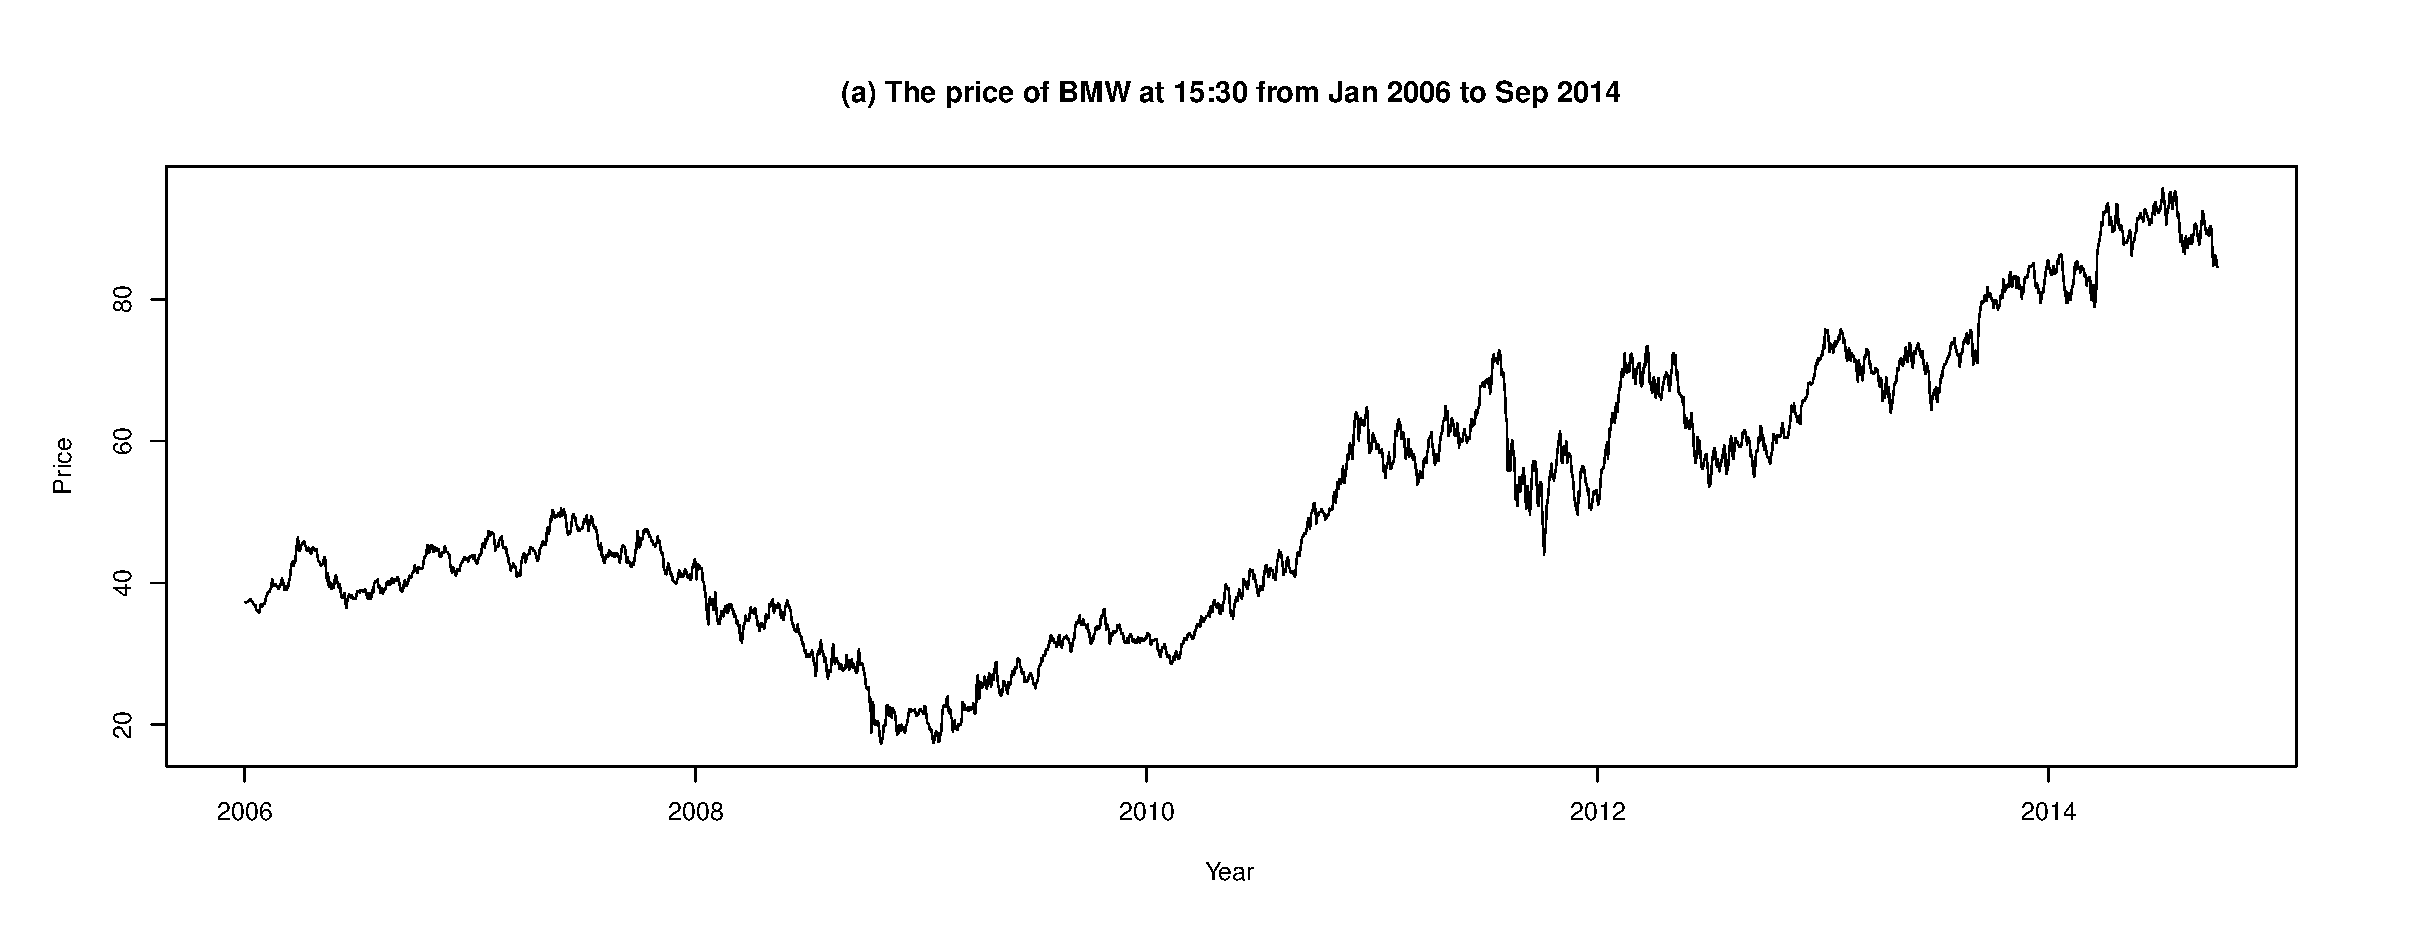
\includegraphics[scale=0.6]{Images/bmw/BMW1530_001.ps}
%%
%%	\label{fig:BMW1530_001}
%%\end{figure}
%
%
%\begin{figure}[t]
%	\centering
%	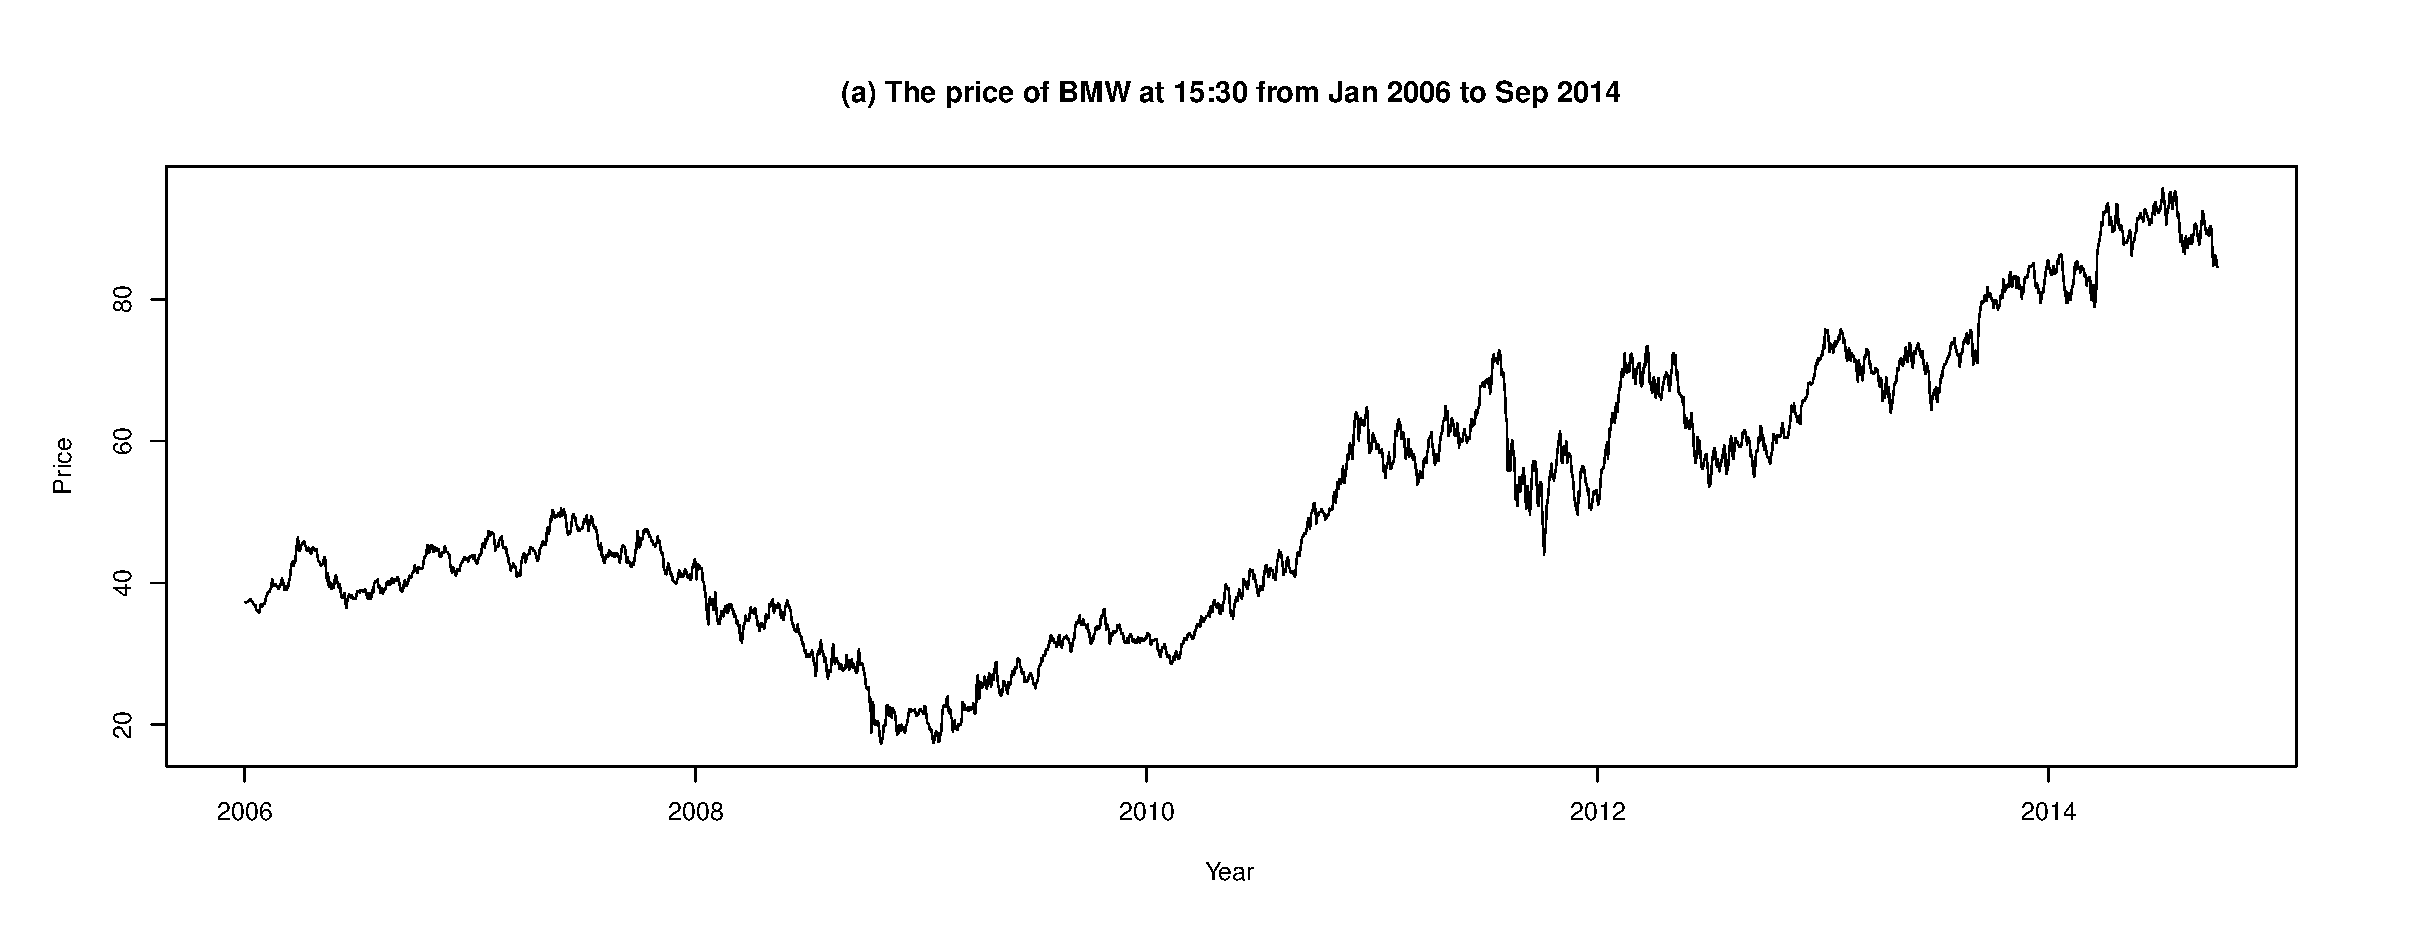
\includegraphics[scale=0.3]{Images/bmw/BMW1530_001}
%	\caption{The price of BMW at 15:30 from Jan 2006 to Sep 2014}
%	\label{fig:BMW1530_001}
%\end{figure}
%
%\begin{figure}[t]
%	\centering
%	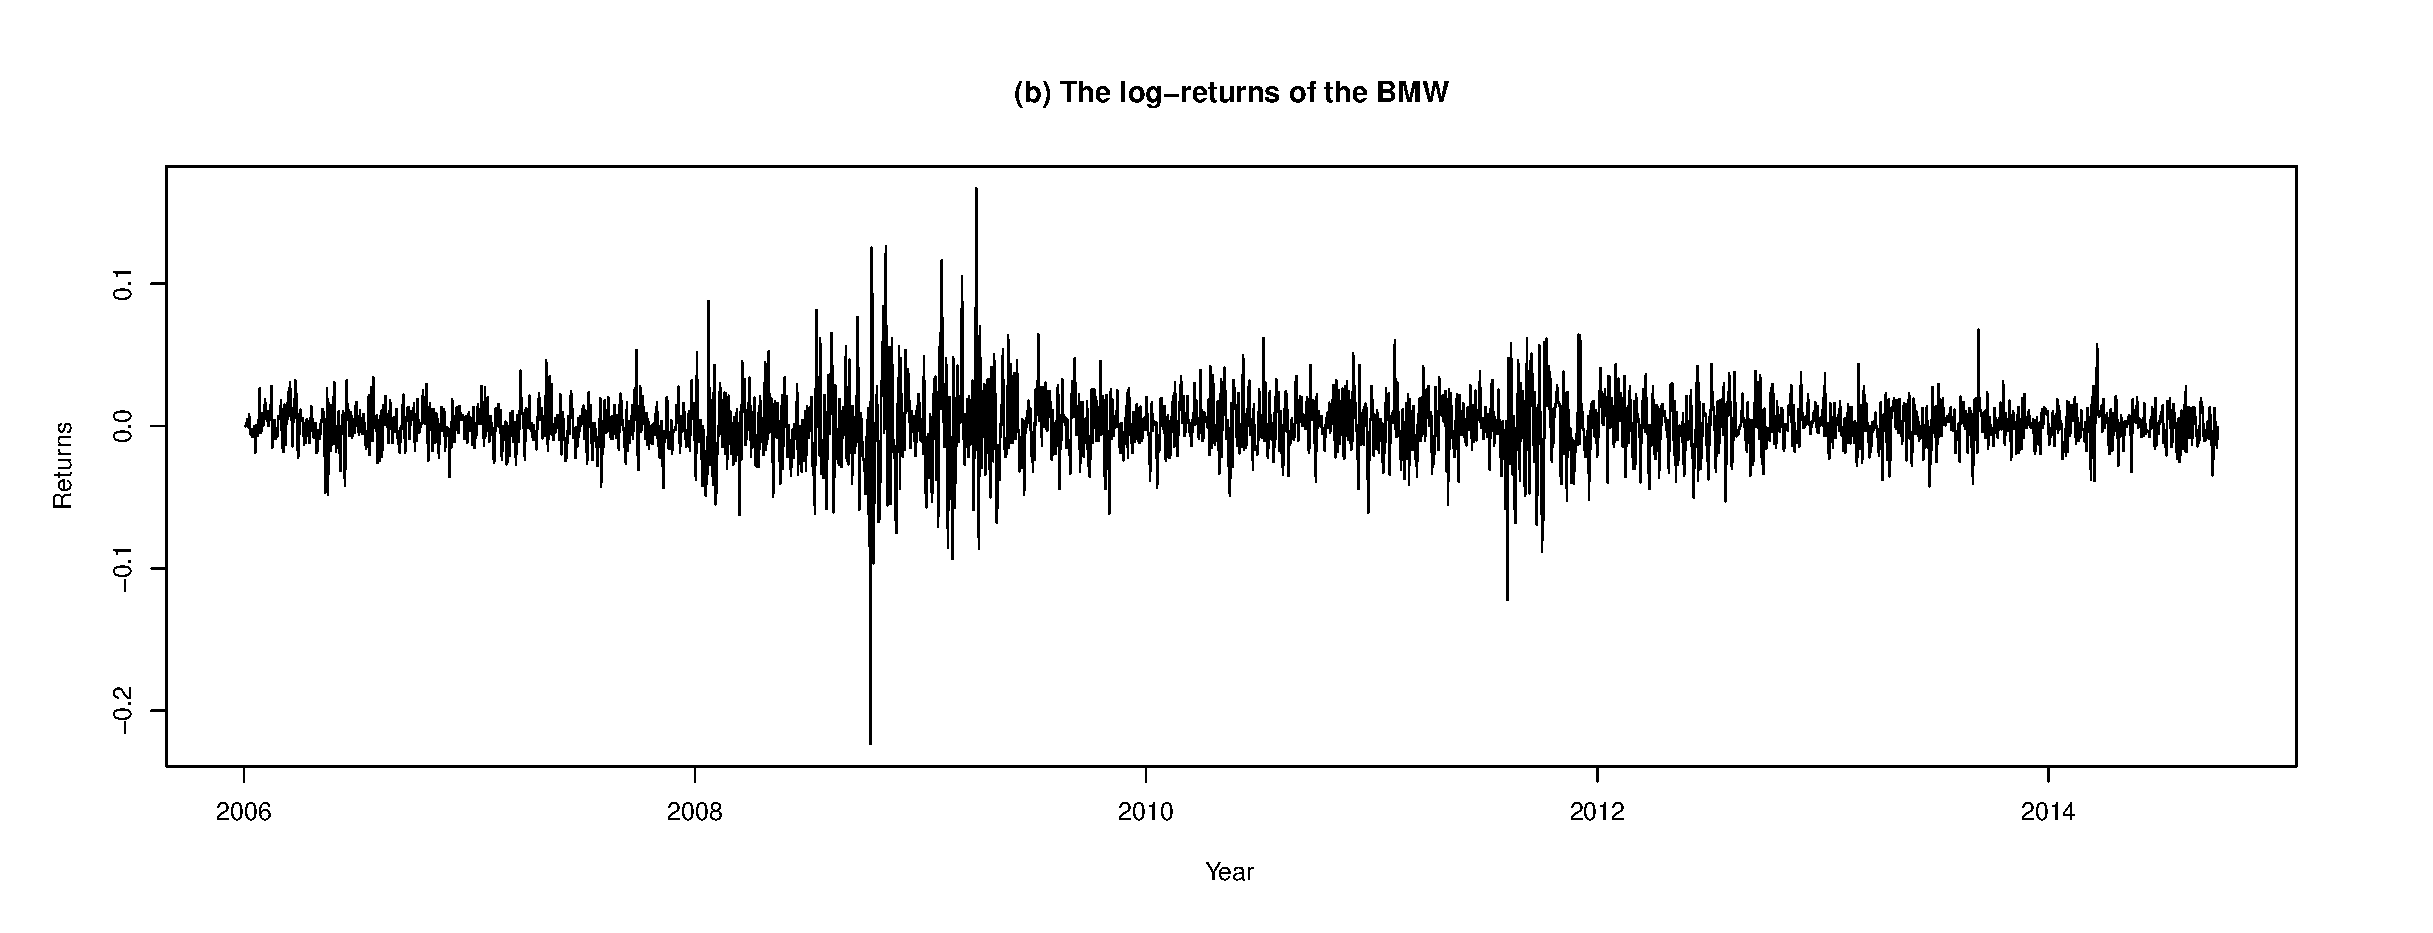
\includegraphics[scale=0.3]{Images/bmw/BMW1530_002}
%	\caption{The log−returns of the BMW}
%	\label{fig:BMW1530_002}
%\end{figure}
%\begin{figure}[t]
%	\centering
%	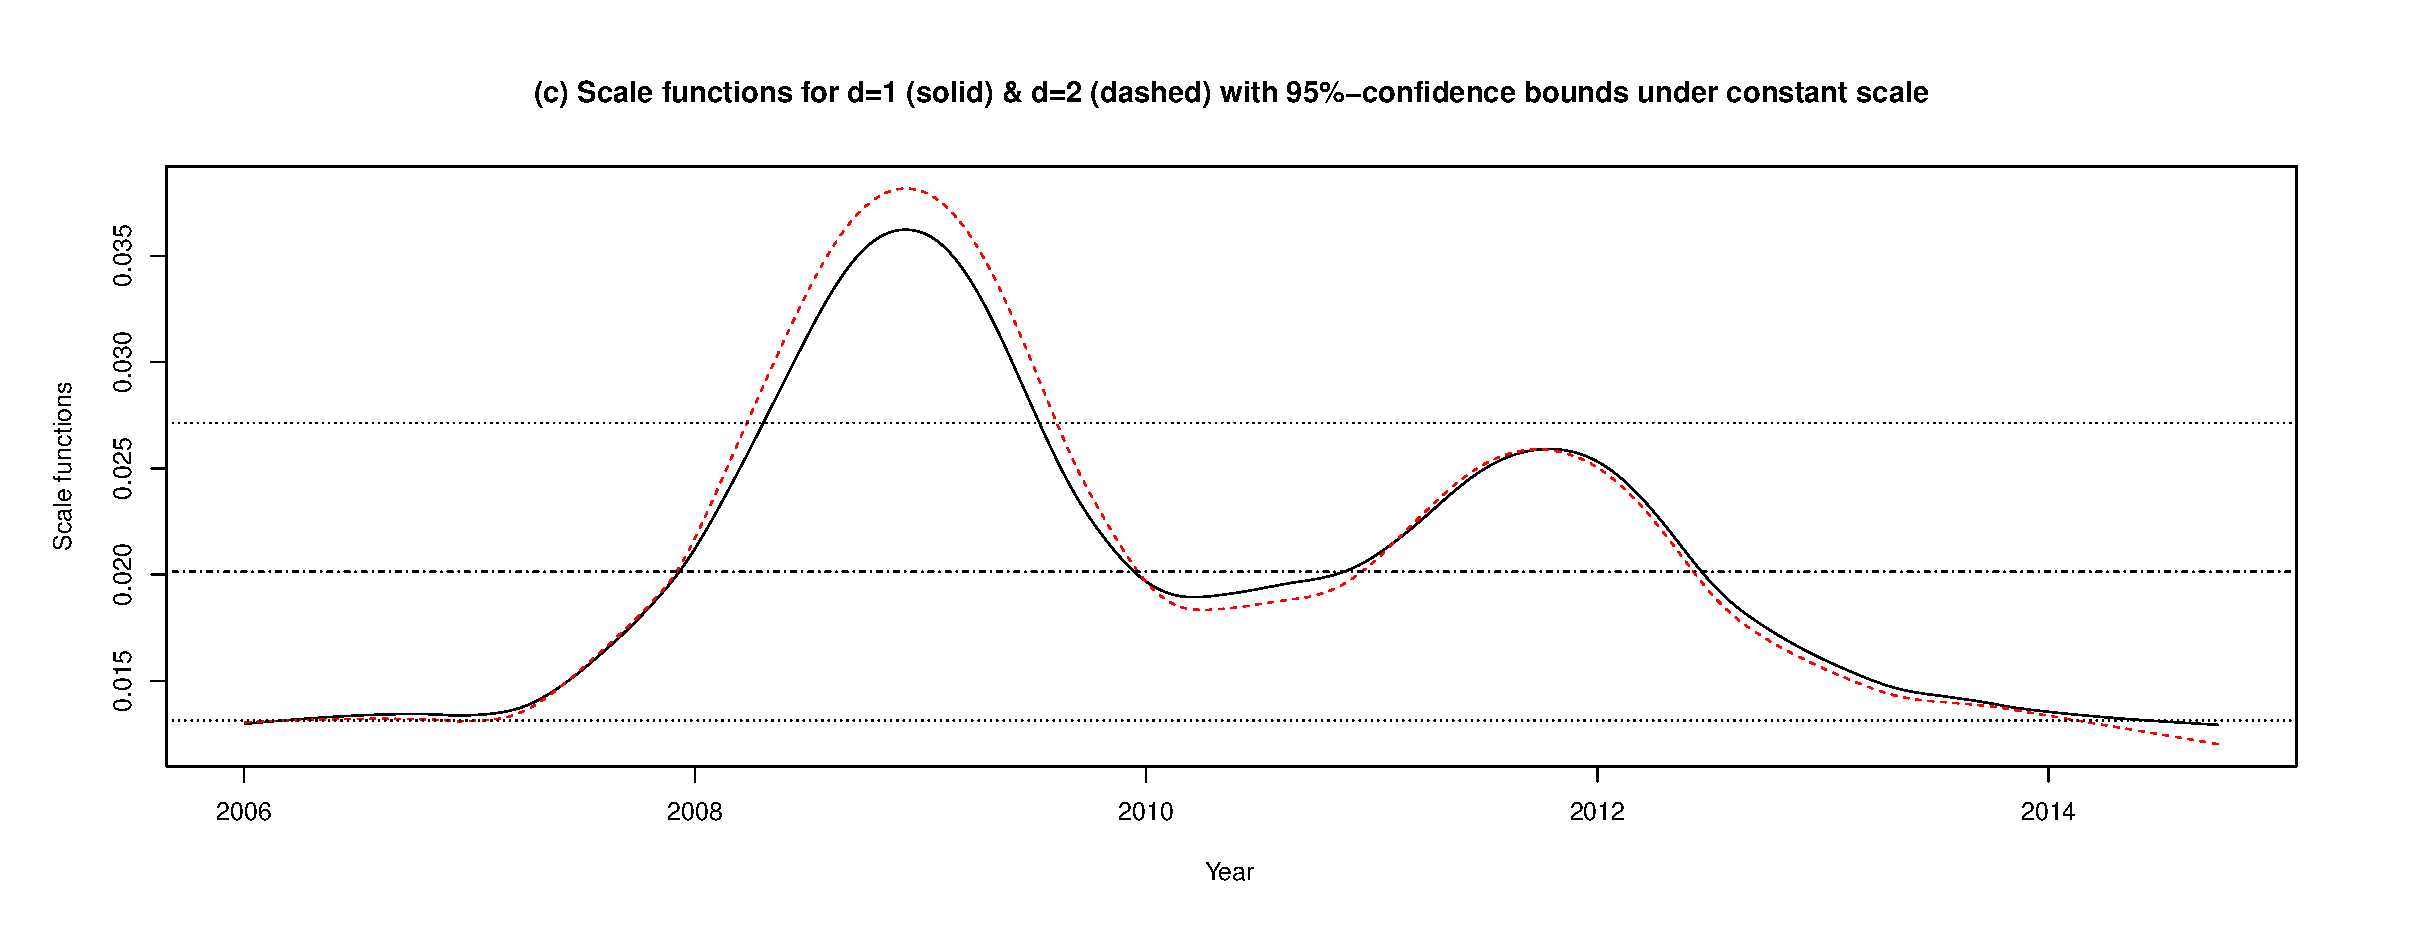
\includegraphics[scale=0.3]{Images/bmw/BMW1530_003}
%	\caption{The price of BMW at 15:30 from Jan 2006 to Sep 2014}
%	\label{fig:BMW1530_003}
%\end{figure}
%\begin{figure}[t]
%	\centering
%	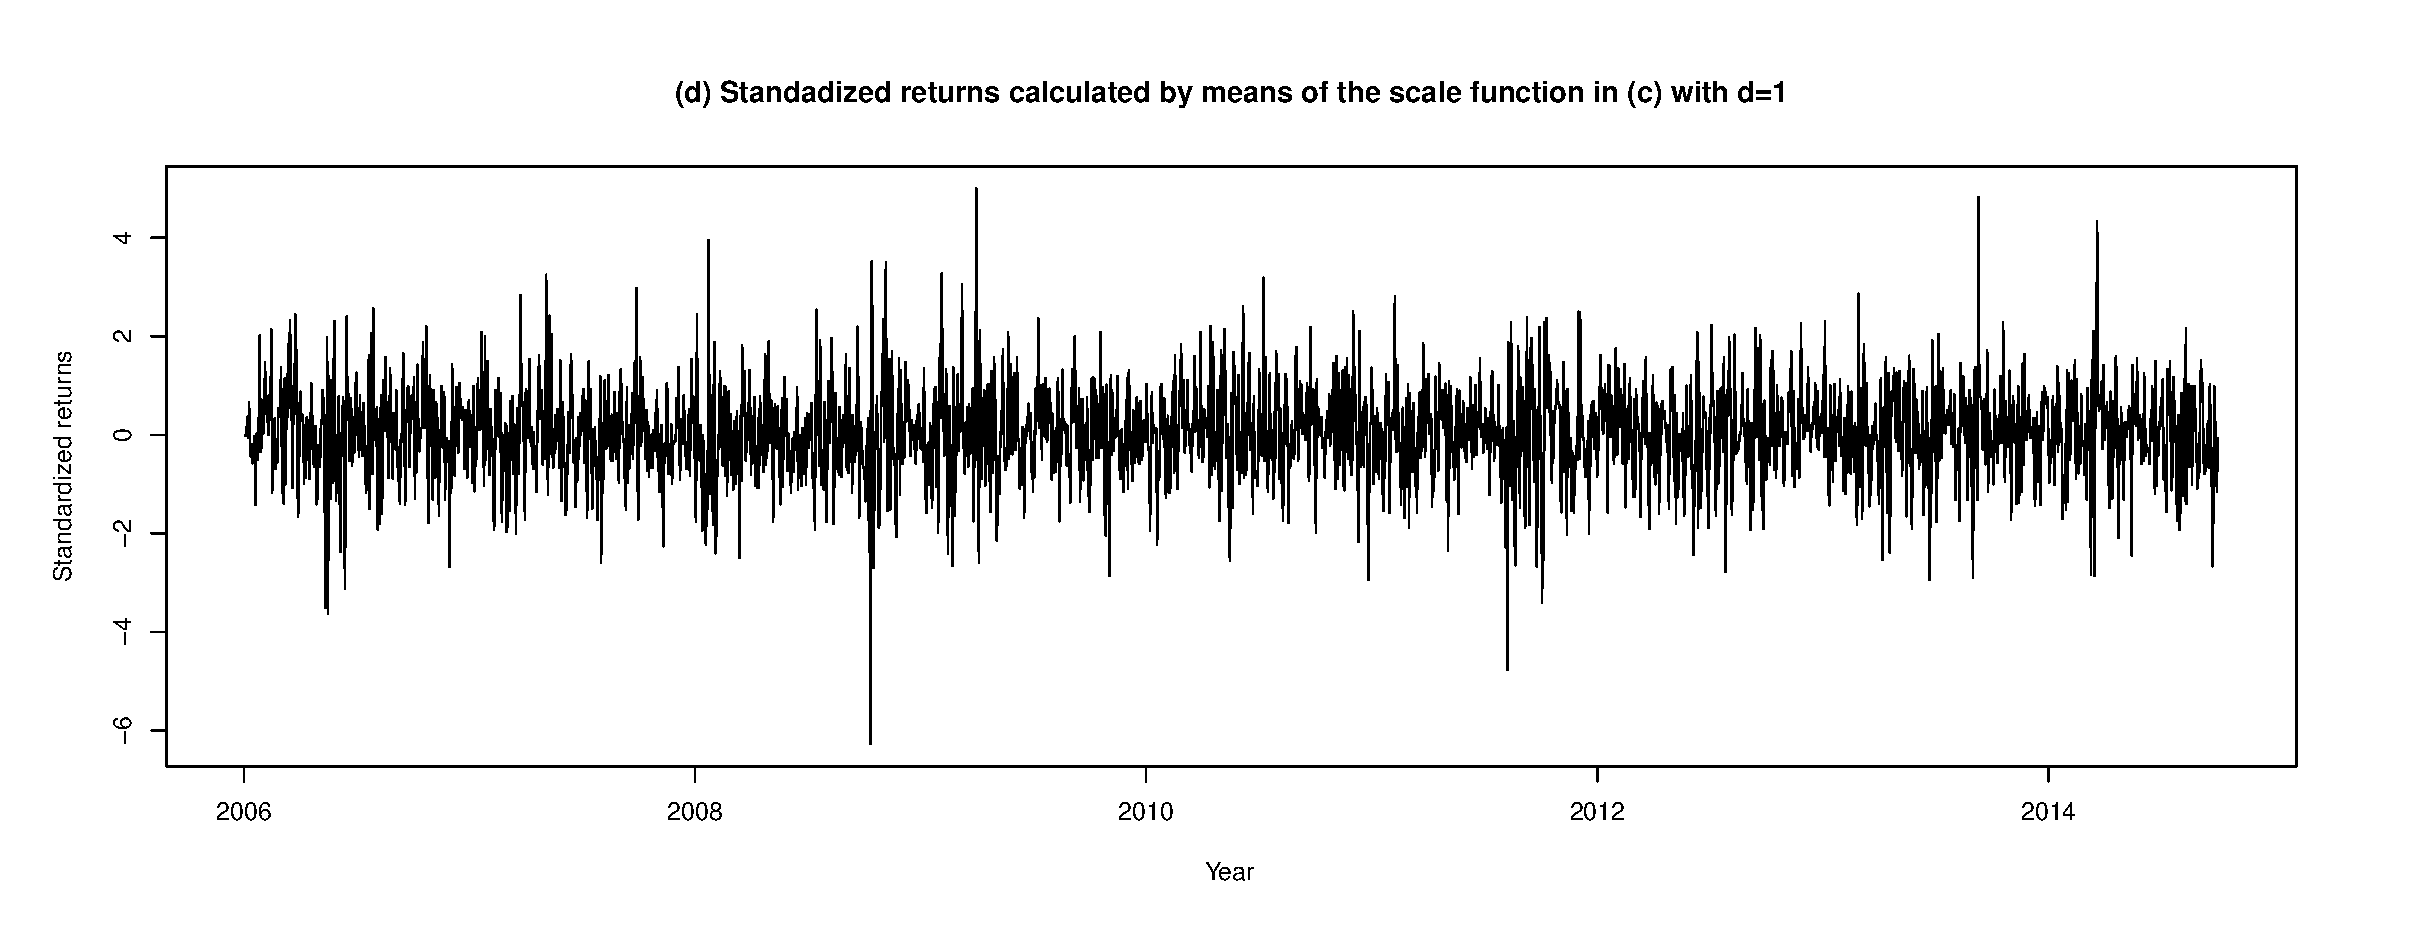
\includegraphics[scale=0.3]{Images/bmw/BMW1530_004}
%	\caption{The price of BMW at 15:30 from Jan 2006 to Sep 2014}
%	\label{fig:BMW1530_004}
%\end{figure}
%
%
